\subsection{Augmentation Patterns}
\label{AugmentPatterns}

\subsubsection{Measurement of Pattern Similarity by Kernels.}
\label{SimKernels}

The kernel methods are a class of algorithm universally used for pattern analysis. The essence of kernel is a similarity that maps a pair of instance to a similarity score. Given a finite set of \textbf{K} instance, the kernel can be represented as a $\textbf{K}\times\textbf{K}$ similarity matrix that contains similarity scores of all pairwise combination of instances.Kernels can be computed simply by computationally-efficient inner products between the images of all pairs of instance, rather than make operation in a much higher dimension of feature spaces such as graphs or trees.

\textbf{Rigid Kernel.} Without loss of completeness and uniformity, we include the case of rigid similarity here by implementing a rigid kernel. According to the definition of rigid similarity (Section \ref{GenPatterns}), The similarity matrix of rigid kernel is a diagonal matrix, that is, elements are equal to one in diagonal and zero for the rest. To be precise, the rigid kernel function \emph{$K_{rigid}$(Pattern\_i,Pattern\_j)} between two pattern is defined as:

\begin{equation}
\begin{aligned}
K_{rigid}(Pattern\_i,Pattern\_j) =
\begin{cases}
 1 & \text{ if } i=j \\
 0 & \text{ if } i\neq j
\end{cases}
\end{aligned}
\end{equation}

\textbf{Shallow Linguistic Kernel. } We define \emph{Shallow Linguistic Kernel} specifically for \emph{Shallow Linguistic Pattern}. Since most of the features defined are incomparable, or at least, difficult for quantification, for example, you cannot tell too hastily the extent to which a pattern \emph{P} with a preposition is different from the pattern without. So we only take into consideration D1 value(number of words between first two elements of a triplet) and D2 value (number of words between last two elements of a triplet) for similarity comparison. Here we borrow the idea of edit distance, to be precise, the shallow linguistic function \emph{$K_{SL}$(Pattern\_i,Pattern\_j)} between two pattern is defined as:

\begin{equation}
\begin{aligned}
K_{SL}(Pattern\_i,Pattern\_j) &= \\
&\begin{cases}
 e^{-\gamma (\triangle D1 + \triangle D2)} & \text{ if } SameOrder \\
 0 & \text{ if } otherwise
\end{cases}
\end{aligned}
\end{equation}

\emph{$\triangle$D1,$\triangle$D2 is the absolute value of D1,D2 difference between $Pattern\_i$,$Pattern\_j$; SameOrder indicates the PPI orders of $Pattern\_i$ and $Pattern\_j$ are identical.} \\

\textbf{Subtree Kernel(ST).} The \emph{subtree kernel} quantify the similarity of two trees through counting all common subtrees\cite{DBLP:conf/nips/ViswanathanS02} (Figure \ref{fig:convKernel}A) in the Tri-Branch Tree representation generated at section \ref{GenPatterns}. Only if the node labels, subtrees and their order are identical would be two trees regarded as the same.

\textbf{Subset Tree Kernel(SST).} The \emph{subset tree kernel} is quite similar to \emph{subtree kernel}, except that it is no longer bound to the restriction that all descendants have to be included in the substructures\cite{DBLP:conf/nips/CollinsD01}. Given a tree node, either none or all of its descendants need to be included in the subset tree (Figure \ref{fig:convKernel}C).

\textbf{Spectrum Tree Kernel(SpT)\cite{Kuboyama07}.} The \emph{spectrum tree kernel} focuses on directed motifs with certain size \emph{k}, called \emph{k-gram}, rather than subtrees\cite{DBLP:conf/nips/CollinsD01} (Figure \ref{fig:convKernel}B). A \emph{spectrum tree} is represented by a set of \emph{k-grams}, usually \emph{k} is 3 or 4. Noticing that the edges are directed, that is, a$\longrightarrow$b$\longrightarrow$c is different from a$\longrightarrow$b$\longleftarrow$c. \\

\begin{figure*}[htb]
\centering
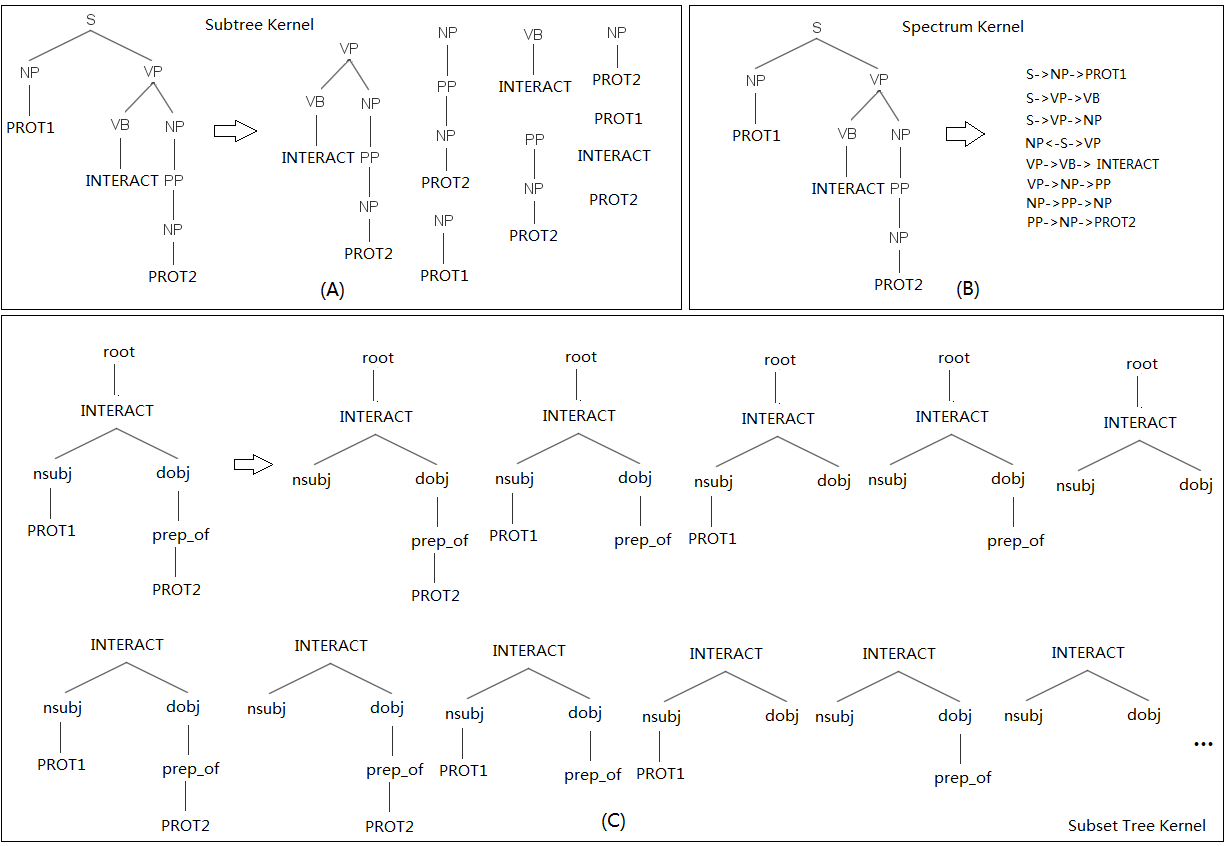
\includegraphics[width=1.0\textwidth]{fig/figure7.png}
\caption{Kernels}
\label{fig:convKernel}
\end{figure*}

After a similarity matrix is defined by kernel functions, for a query pattern, the simplest and most natural choice is to find \emph{k} nearest neighbor patterns by looking after those patterns with highest similarity scores; Alternatively, we could find out all those patterns of which the similarity scores exceed some minimum similarity threshold $\mathcal {T}_{sim}$. Finally, we add new patterns associated with similarity to the candidate pattern sets for further evaluation.

\subsubsection{Evaluation of Augmented Patterns}
The evaluation of those augmented patterns is crucial, for the reasons that additional qualified patterns would transcend the limited size and narrow coverage of original candidate pattern set and thus contribute to the diversity of results of tuple extraction at last; on the other hand, if those "bad" patterns escape from filtering and play the role of extracting new tuples, then performance would be jeopardized, what's even worse, less satisfactory than the situation without applying pattern augmentation.

The confidence of an augmented pattern is twofold: first, according to the essence of pattern evaluation (Section \ref{EvalPatterns}), all triplets matching one specific pattern are put together to contribute to the confidence of certain pattern; second, since the augmented patterns are achieved due to an original one by similarity, so their confidences should be highly related to the confidence of original pattern in some sense. Also, chances are high that an newly-augmented pattern already exists actually, in that case, the confidence of that pattern should be enhanced for its validity is proved by similar counterparts. Finally, we believe augmented patterns less than those directly generated by seed tuples, so we downgrade the importance of augmented patterns to some extent. Consider an augmented Pattern \emph{$P_{aug}$}, and it is induced by original Pattern \emph{$P_{origin}$} based on similarity \emph{sim}, then we calculate the confidence of the augmented Pattern \emph{$P_{aug}$} based on algorithm \emph{CALCULATE-AUGPATTERN-CONF}:

%\begin{equation}
%\begin{aligned}
%Conf_{aug}(P_{aug})&=\bbbeta *(W_{own}*Conf(P_{aug}) \\
%        &+ (1-W_{own})*sim*Conf(P_{origin}))
%\end{aligned}
%\end{equation}

\begin{codebox}
\Procname{$\proc{Calculate-AugPattern-Conf($P_{aug}, P_{origin}, sim$)}$}
\li $conf \gets 0$
\li \If $P_{aug}$ already exists
\li     \Then
            $conf \gets Conf(P_{aug})$
        \End
\li $newConf \gets \bbbeta *(W_{own}*Conf(P_{aug})$\zi \space\space\space\space\space\space\space $+(1-W_{own})*sim*Conf(P_{origin}))$
\li $conf \gets conf+newConf$
\li \Return $conf$
\end{codebox}

The parameter $W_{own}$ represents for the augmentation rate. If $W_{own}>0.5$ then the \emph{PPISnowball} system in effect trusts more in the own confidence brought from corresponding triplets, shown as $Conf(P_{aug})$, which will lead to more independent patterns and have a diversified effect; else if $W_{own}<0.5$ then the \emph{PPISnowball} system appears to trusts more in the derived confidence resulting from similarity associations, shown as $sim*Conf(P_{origin})$, which will lead to more interdependent patterns and have a clustering effect. For our experiments, we set $W_{own}=0.5$. Besides, the parameter $\bbbeta$ is a numeric number, ranging from 0 to 1. It downgrades the importance of augmented patterns in terms of confidence. If a newly-augmented pattern already exists, the confidence would be accumulated.


